\documentclass[12pt]{article}

\usepackage{amsmath}
\usepackage{mathtools}
\usepackage{bigints}
\usepackage{parskip}
\usepackage{color}
\usepackage{amssymb}

    \newenvironment{myindentpar}[1]%
     {\begin{list}{}%
             {\setlength{\leftmargin}{#1}}%
             \item[]%
     }
     {\end{list}}

\begin{document}
\title{Final Exam Study Guide}
\date{Final Exam Date \& Location: Thursday May 15 8:00pm - 10:00pm MacBride Auditorium}
\author{}
\maketitle

{\Large \textbf{NOTE:} The final exam is \textbf{CUMULATIVE}. Make sure you study everything we've done this semester and not just the material since the previous midterm.}

\section{Matrices \& Solving Linear Systems}

\textbf{Matrix:}

\begin{itemize}
\item a \textit{matrix} is a rectangular array of numbers
\item the \textit{dimension} of a matrix is the number of rows ($m$) by the number columns ($n$). A general matrix with $m$ rows and $n$ columns has dimension $m \times n$. \textbf{Dimension:} (\# of Rows) $\times$ (\# of Columns)
\item matrices allow us to succinctly represent a large amount of information
\end{itemize}

\vspace{1cm}

\textbf{Matrix Algebra:} 

\begin{itemize}
\item \textbf{Addition:} Given two matrices $A$, $B$ of the same dimension then the sum $A + B$ is the matrix obtained by adding the corresponding entries in the two matrices
\begin{myindentpar}{1cm}
Example: 

$\begin{bmatrix}                                        
       1 & 2 & 0           \\[1em]			
       -5 & 0           & 3 \\[1em]       		
       2           & -3 & -6				
     \end{bmatrix}$
+ 			 
$\begin{bmatrix}                                        
       -3 & 7 & -2           \\[1em]			
       0 & 4           & -2 \\[1em]       		
       5           & -1 & 2				
     \end{bmatrix}$
= 
$\begin{bmatrix}                                        
       -2 & 9 & -2           \\[1em]			
       -5 & 4           & 1 \\[1em]       		
       7           & -4 & -4				
     \end{bmatrix}$
\end{myindentpar}
\item \textbf{Subtraction:} Given two matrices $A$, $B$ of the same dimension then the difference $A - B$ is the matrix obtained by subtracting the corresponding entries in the two matrices
\item \textbf{Scalar Multiplication:} Given a matrix $A$ and a number $c$ then the product $cA$ is the matrix obtained by multiplying each entry of $A$ by $c$
\end{itemize}


\begin{myindentpar}{1cm}
Example:

2 $\cdot \begin{bmatrix}                                        
       1 & 2 & 0           \\[1em]			
       -5 & 0           & 3 \\[1em]       		
       2           & -3 & -6				
     \end{bmatrix}$
= 
$\begin{bmatrix}                                        
       2 & 4 & 0           \\[1em]			
       -10 & 0           & 6 \\[1em]       		
       4           & -6 & -12				
     \end{bmatrix}$
\end{myindentpar}

\vspace{1cm}

\textbf{Matrix Multiplication:}

\begin{itemize}
\item Given two matrices, $A$, $B$, we can also find the matrix product $AB$, but we need to be careful. Matrix multiplication is NOT ALWAYS possible.
\item Given two matrices $A$, $B$ we can find the matrix product, $AB$, if the \textbf{number of columns of A is equal to the number of rows in B}
\item Given a matrix $A$ of dimension $(m \times n)$ and a matrix $B$ of dimension $(n \times k)$ AB will be a matrix of dimension $(m \times k)$
\item So if we are multiplying a $(\textcolor{red}{m} \times \textcolor{blue}{n})$ matrix $A$ by a $(\textcolor{blue}{n} \times \textcolor{red}{k})$ matrix $B$. The inner numbers (the numbers in \textcolor{blue}{blue}) will tell you whether or not matrix multiplication is possible. If it is possible, the outer numbers (numbers in \textcolor{red}{red}) tell you the dimension of the matrix AB

\begin{myindentpar}{1cm}
Example:

A = $\begin{bmatrix}                                        
       1 & 3 & -2           \\[1em]			
       -1 & 1           & 4 \\[1em]       		
       3          & 0 & -3 \\[1em]	
       2          & -4 & -6			
     \end{bmatrix}$ \hspace{1cm}
B = $\begin{bmatrix}                                        
       -1 & 2 & 0           \\[1em]			
       -5 & 2           & 3 \\[1em]       		
       0          & -1 & -3				
     \end{bmatrix}$

\vspace{1cm}

\centerline{
AB = $\begin{bmatrix}                                        
       1(-1) + 3(-5) + -2(0) & 1(2) + 3(2) + -2(-1) & 1(0) + 3(3) + -2(-3)           \\[1.5em]			
       -1(-1) + 1(-5) + 4(0) & -1(2) + 1(2) + 4(-1)           & -1(0) + 1(3) + 4(-3) \\[1.5em]       		
       3(-1) + 0(-5) + -3(0)          & 3(2) + 0(2) + -3(-1) & 3(0) + 0(3) + -3(-3)  \\[1.5em]   
       2(-1) + -4(-5) + -6(0)          & 2(2) + -4(2) + -6(-1) & 2(0) + -4(3) + -6(-3)			
     \end{bmatrix}$}

\vspace{1cm}

\centerline{
= $\begin{bmatrix}                                        
       -16 & 10& 15           \\[1.5em]			
       -4& -4 & -9 \\[1.5em]       		
       -3 & 9 & 9   \\[1.5em]   
       18 & 2 & 6			
     \end{bmatrix}$
}
\end{myindentpar}

\textbf{Note:} To find the entry in the \textbf{\textcolor{red}{first row}}, \textbf{\textcolor{blue}{first column}} of AB we multiply the corresponding entries of the \textbf{\textcolor{red}{first row of A}} by the \textbf{\textcolor{blue}{first column of B}} and add them all up.

To find the entry in the \textbf{\textcolor{red}{first row}}, \textbf{\textcolor{blue}{second column}} of AB we multiply the corresponding entries of the \textbf{\textcolor{red}{first row of A}} by the \textbf{\textcolor{blue}{second column of B}} and add them all up

We can continue on in this fashion:

i.e. To find the...

\textbf{\textcolor{red}{First row}}, \textbf{\textcolor{blue}{third column}} of AB $\rightarrow$ multiply the \textbf{\textcolor{red}{first row of A}} by the \textbf{\textcolor{blue}{third column of B}} and add

\textbf{\textcolor{red}{First row}}, \textbf{\textcolor{blue}{fourth column}} of AB $\rightarrow$ multiply the \textbf{\textcolor{red}{first row of A}} by the \textbf{\textcolor{blue}{fourth column of B}} and add

\textbf{\textcolor{red}{Second row}}, \textbf{\textcolor{blue}{first column}} of AB $\rightarrow$ multiply the \textbf{\textcolor{red}{second row of A}} by the \textbf{\textcolor{blue}{first column of B}} and add

etc...

\end{itemize}

\textbf{Identity Matrix:}
\begin{itemize}
\item the \textbf{Identity Matrix} is a special type of matrix with $1's$ along the main diagonal and zeros everywhere else
\item it is always a square matrix (the number of rows = number of columns of the identity matrix)
\item given a matrix $A$ and the identity matrix $I$, the product of $AI = A$ (provided they are of appropriate dimension). So to give an analogy, multiplying a matrix by the identity matrix is like multiplying a number times $1$
\end{itemize}

\vspace{.5cm}

\begin{myindentpar}{1cm}
\centerline{
\textbf{3x3 Identity Matrix:}}
\vspace{.5cm}
\centerline{
$\begin{bmatrix}                                        
       1 & 0& 0           \\[.5em]			
       0& 1 & 0 \\[.5em]       		
       0 & 0 & 1   		
     \end{bmatrix}$}
\end{myindentpar}

\textbf{Solving Linear Systems}
\begin{itemize}
\item We learned how to solve two types of linear systems: 

\begin{enumerate}

\item $2$ equations and $2$ unknowns
\newline

\centerline{$a_{1,1}x + a_{1,2}y = b_{1}$}

\vspace{.3cm}

\centerline{$a_{2,1}x + a_{2,2}y = b_{2}$}

\textbf{Note:} These are merely equations of lines. (Any two points $x$ and $y$ determine a line)
\item $3$ equations and $3$ unknowns:
\newline

\centerline{$a_{1,1}x + a_{1,2}y + a_{1,3}z  = b_{1}$}

\vspace{.3cm}

\centerline{$a_{2,1}x + a_{2,2}y + a_{2,3}z  = b_{2}$}

\vspace{.3cm}

\centerline{$a_{3,1}x + a_{3,2}y + a_{3,3}z = b_{3}$}

\textbf{Note:} These are equations of planes. (Any three points $x$, $y$, and $z$ determine a plane)
\end{enumerate}

\item For a (2 by 2) or a (3 by 3) system the solution will be one of three possibilities:
\begin{enumerate}
\item There will be one and only one solution
\item There will be an infinite number of solutions
\item There will be no solution
\end{enumerate}

Visually, this is what is going on in the (2 by 2) case:

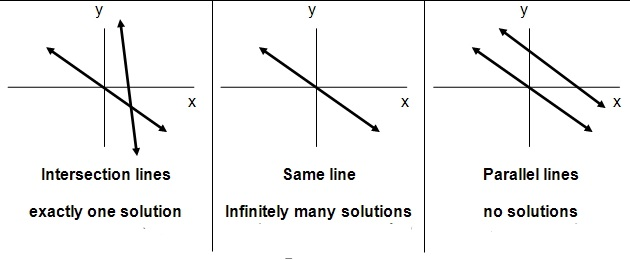
\includegraphics[scale=.7]{LinearSystemSoln.jpg}

Visually, this is what is going on in the (3 by 3) case:

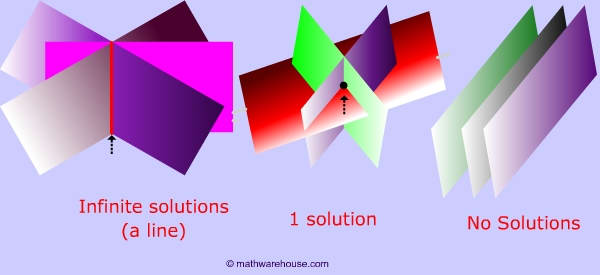
\includegraphics[scale=.5]{LinearSystemSolution3By3.jpg}

\item to solve a linear system we learned two methods: 

\begin{enumerate}
\item\textbf{Gaussian Elimination} 
\item\textbf{Inverse Matrix Method}
\end{enumerate}
Both methods are very similar and they involve augmented matrices and performing row operations on the augmented matrix
\end{itemize}


\textbf{Row Operations}
\begin{enumerate}
\item Interchange any two rows
\item Multiply any row by a nonzero number
\item Add or subtract a multiple of any row to another row
\end{enumerate}

\vspace{1cm}
\newpage

\textbf{Example of Gaussian Elimination:}

\centerline{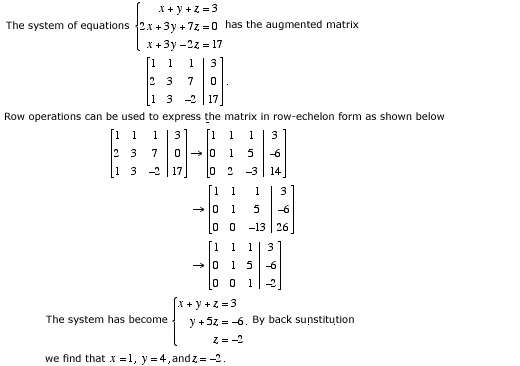
\includegraphics{GaussianElimination.jpg}}

\newpage

\textbf{Inverse Matrix Method:}

\begin{itemize}
\item Given a linear system of $3$ equations and $3$ unknowns:
\newline

\centerline{$a_{1,1}x + a_{1,2}y + a_{1,3}z  = b_{1}$}

\vspace{.3cm}

\centerline{$a_{2,1}x + a_{2,2}y + a_{2,3}z  = b_{2}$}

\vspace{.3cm}

\centerline{$a_{3,1}x + a_{3,2}y + a_{3,3}z = b_{3}$}

\item we can write this in \textbf{matrix form} $AX = B$:
\newline

\centerline{
$\begin{bmatrix}                                        
       a_{1,1} & a_{1,2}& a_{1,3}           \\[1em]			
       a_{2,1}& a_{2,2} & a_{2,3} \\[1em]       		
       a_{3,1} & a_{3.2} & a_{3,3}   \\		
     \end{bmatrix}$
$\begin{bmatrix}                                        
       x           \\[1em]			
       y  \\[1em]       		
       z \\		
     \end{bmatrix}$
$= \begin{bmatrix}                                        
       b_{1}           \\[1em]			
       b_{2}  \\[1em]       		
       b_{3} \\		
     \end{bmatrix}$}

\item to solve this we want to find the inverse matrix of $A$ which we denote by $A^{-1}$. Once we have $A^{-1}$ we multiply $A^{-1}B$ which gives us $X$. 

\item the general idea is to start with an augmented matrix with the matrix of coefficients ($A$) on the left and the ($3 \times 3$) Identity matrix on the right:

\[
\left[
\begin{array}{ccc|ccc}
a_{1,1} & a_{1,2} & a_{1,3} & 1 & 0 & 0 \\
a_{2,1} & a_{2,2} & a_{2,3} & 0 & 1 & 0 \\
a_{3,1} & a_{3,2} & a_{3,3} & 0 & 0 & 1 \\
\end{array}
\right]
\]

and then perform a bunch of row operations to get it in the form:

\[
\left[
\begin{array}{ccc|ccc}
1 & 0 & 0 & a_{1,1}^{-1} & a_{1,2}^{-1} & a_{1,3}^{-1} \\[1em]
0 & 1 & 0 & a_{2,1}^{-1} & a_{2,2}^{-1} & a_{2,3}^{-1} \\[1em]
0 & 0 & 1 & a_{3,1}^{-1} & a_{3,2}^{-1} & a_{3,3}^{-1} \\
\end{array}
\right]
\]

where we now have the ($3 \times 3$) Identity matrix on the left and the inverse matrix ($A^{-1}$) is on the right. See the following page for an example of how to find the inverse of a matrix $A$.
\end{itemize}

\textbf{Example of Inverse Matrix Method:}

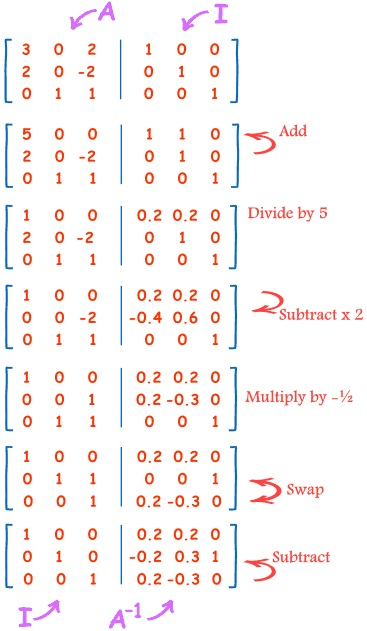
\includegraphics{InverseMatrixMethod.jpg}

\section{Set Theory \& Probability Theory}

\textbf{Sets}

\begin{itemize}
\item a \textit{set} is a collection of objects
\item the \textbf{empty set} is the set containing no elements and is denoted as $\emptyset$
\end{itemize}

\vspace{.5cm}

\textbf{Subsets}

\begin{itemize}
\item a set $A$ is a \textit{subset} of a set $B$ if every element of $A$ is also an element of $B$
\item if $A$ is a subset of $B$ then we denote it by $A \subseteq B$
\end{itemize}

\begin{myindentpar}{2cm}
\textbf{Example:} Let $A = \{a,c,e,g\}$ and $B = \{a,b,c,d,e,f,g\}$

Then $A \subseteq B$ since every element of $A$ is also in $B$

\end{myindentpar}


\centerline{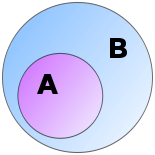
\includegraphics[scale=.5]{Subset.png}}

\vspace{.5cm}

\textbf{Union} - given two sets $A$, $B$, the \textit{union} is the collection of elements in both $A$ \textbf{or} $B$ denoted by $A \cup B$ 
\newline

\centerline{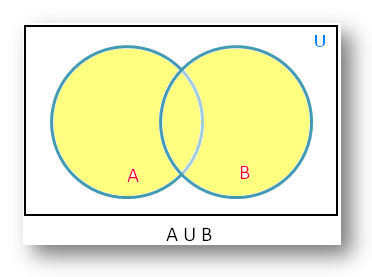
\includegraphics[scale=.5]{Union.png}}

\textbf{Note:} Same definition holds for two events, $E$ \& $F$, in a sample space $S$

\textbf{Intersection} - given two sets $A$, $B$, the \textit{intersection} is the collection of elements in both $A$ \textbf{and} $B$ denoted by $A \cap B$
\newline

\centerline{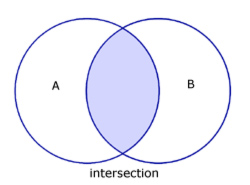
\includegraphics[scale=.7]{Intersection.jpg}}

\textbf{Note:} The same definition holds for two events, $E$ \& $F$, in a sample space $S$

\vspace{.5cm}

\textbf{Complement} - given a set $A$ the \textit{complement} of $A$  is the collection of elements \textbf{not in} $A$ denoted by $A^{c}$
\newline

\centerline{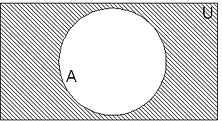
\includegraphics{Complement.png}}

\textbf{Note:} The same definition holds for an event, $E$, in a sample space $S$

\vspace{1.5cm} 

\textbf{Properties of Set Operations:}

\begin{enumerate}
\item $A \cup B = B \cup A$ \hspace {4cm} (Union is commutative)
\item $A \cap B = B \cap A$ \hspace {4cm} (Intersection commutative)
\item $A \cup (B \cup C) = (A \cup B) \cup C$ \hspace {1.8cm} (Union is associative)
\item $A \cap (B \cap C) = (A \cap B) \cap C$ \hspace {1.8cm} (Intersection is associative)
\item $A \cup (B \cap C) = (A \cup B) \cap (A \cup C)$ \hspace {.65cm} (Distributive Law for Union)
\item $A \cap (B \cup C) = (A \cap B) \cup (A \cap C)$ \hspace {1cm} (Distributive Law for Intersection)
\end{enumerate}

\vspace{.5cm}

\textbf{De Morgan's Laws:}

\begin{enumerate}
\item $(A \cup B)^{c} = A^{c} \cap B^{c}$
\item $(A \cap B)^{c} = A^{c} \cup B^{c}$
\end{enumerate}

\vspace{.5cm}

\textbf{Generalized Multiplication Principle:}

\begin{myindentpar}{2cm}
Suppose a task $T_{1}$ can be performed in $N_{1}$ ways, a task $T_{2}$ can be performed in $N_{2}$ ways, a task $T_{3}$ can be performed in $N_{3}$ ways,..., and, finally, a task $T_{m}$ can be performed in $N_{m}$ ways. Then the number of ways of performing the tasks $T_{1}, T_{2}, T_{3},...,T_{m}$ in succession is given by:
\newline

\centerline{$N_{1} \cdot N_{2} \cdot N_{3} \cdot \cdots \cdot N_{m}$}
\end{myindentpar}

\vspace{.5cm}

\textbf{n-Factorial:}
For any natural number $n$, the \textit{n-factorial} is given by
\newline

\centerline{$n! = n \cdot (n-1) \cdot (n-2) \cdot (n-3) \cdots 3 \cdot 2 \cdot 1$}

\hspace{5cm} with $0! = 1$

\vspace{.5cm}

\textbf{Permutation of n Distinct Objects:} 

The number of permutations of $n$ objects taken $r$ at a time is given by:
\newline

\centerline{$P(n,r) = \dfrac{n!}{(n-r)!}$}


With permutations, \textbf{ORDER MATTERS}

\vspace{.5cm}

\textbf{Permutation of n Objects (Not all Distinct):}

Given a set of $n$ objects in which $n_{1}$ objects of one kind are alike, $n_{2}$ objects of another kind are alike, $n_{3}$ objects of another kind are alike,...,$n_{m}$ objects of another kind are alike then the number of permutations of these $n$ taken $n$ at a time is:
\newline

\centerline{$P(n,n_{1},n_{2},n_{3},...,n_{m}) = \dfrac{n!}{n_{1}! \cdot n_{2}! \cdot n_{3}! \cdots n_{m}!}$}


\vspace{.5cm}

\textbf{Combination of n Distinct Objects:} 

The number of combinations of $n$ objects taken $r$ at a time is given by:
\newline

\centerline{$C(n,r) = \dfrac{n!}{r!(n-r)!}$}

\vspace{.5cm}

With combinations, \textbf{ORDER DOESN'T MATTER}

\vspace{.5cm}


\textbf{Probability of Simple Events:}

Let $S$ be a sample space consisting of the following \textbf{simple} events:
\newline

\centerline{$S = \{s_{1}, s_{2}, s_{3}, \dots s_{n}\}$}

Then the following three conditions hold

\begin{enumerate}
\item $0 \leq P(s_{i}) \leq 1$ \hspace{4.3cm} for $i = 1, 2, 3 \cdots, n$
\item $P(s_{1}) + P(s_{2}) + P(s_{3}) + \cdots + P(s_{n}) = 1$
\item $P(s_{i} \cup s_{j}) = P(s_{i}) + P(s_{j})$ \hspace{2cm} for $ i \neq j$ 
\end{enumerate}

\begin{myindentpar}{1cm}\textbf{Note:} The first two conditions ALWAYS hold for any sample space $S$. The probability of any one event will ALWAYS be between $0$ and $1$ (Condition 1) and the probability of the entire sample space will ALWAYS be equal to $1$ (Condition 2).

 The last condition (Condition 3) only holds because the events are \textbf{simple} events which means they are \textbf{mutually exclusive} in that given two events of the sample space $S$ only one can occur at a time. If two events, $E$ \& $ F$, are mutually exclusive then $P(E \cap F) = 0$. This is not always the case.
\end{myindentpar}

\vspace{1cm}
\textbf{Mutually Exclusive Events} - two events $E$, $F$ are \textit{mutually exclusive} if they cannot occur simultaneously. In other words, this means $P(E \cap F) = 0$


\textbf{Probability of an Event in Uniform Space} - if $S$  is a uniform sample space, then the probability that an event $E$ will happen is given by
\newline

\centerline{$P(E) = \dfrac{\text{Number of Outcomes in E}}{\text{Total Number of Outcomes in S}}$}
\vspace{.5cm}

Let's do some examples to highlight what this all means:
\begin{myindentpar}{1cm}
\textbf{Example 1:} Let $S = \{s_{1}, s_{2}, s_{3}, s_{4}, s_{5}, s_{6}\}$ be the sample space associated with the experiment having the following probability distribution of simple events:

\centerline{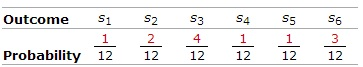
\includegraphics{ProbDistribution.jpg}}
\begin{myindentpar}{1cm}
\textbf{(a)} Find the probability of $A = \{s_1, s_3\}$

Since these are \textbf{simple events} which means they are \textbf{mutually exclusive} then the probability that A occurs is given by

$P(A) = P(s_1 \cup s_3) = P(s_1) + P(s_3) = \dfrac{1}{12} + \dfrac{4}{12} = \dfrac{5}{12}$

\textbf{(b)} Find the probability of $B = \{s_2, s_4, s_5, s_6\}$

Again these are simply events so that $P(B) = P(s_2) + P(s_4) + P(s_5) + P(s_6) = \dfrac{2}{12} + \dfrac{1}{12} + \dfrac{1}{12} + \dfrac{3}{12} = \dfrac{7}{12}$

\textbf{(c)} Find the probability of $C = S$.

Now $S$ is the whole sample space and we know the probability of the entire sample space is ALWAYS equal to $1$ so $P(C) = P(S) = 1$
\end{myindentpar}

\textbf{Example 2:} If a ball is selected at random from an urn containing six red balls, four white balls, and ten blue balls, what is the probability that it will be a white ball? 
\begin{myindentpar}{1cm}
\textbf{Answer:} There are a total of 20 balls in the urn and there are 4 white balls in the bag so we know the probability of choosing a white ball out of the urn is given by the number of ways we can pick a white ball (4) over the total number of balls in the urn (20) so...

$P(\text{Choosing a White Ball})  = \dfrac{4}{20} = \dfrac{1}{5} = 0.2$
\end{myindentpar}
\end{myindentpar}

\vspace{.5cm}

\textbf{Conditional Probability:} If $A$ and $B$ are events in an experiment and $P(A) \neq 0$ then the \textit{conditional probabiity} that the event $B$ will occur given that the event $A$ has already occurred is 
\newline

\centerline{$P(B|A) = \dfrac{P(A \cap B)}{P(A)}$}

\textbf{Probability Rules:}

\begin{enumerate}
\item $P(A \cup B) = P(A) + P(B) - P(A \cap B)$ (\textbf{Addition Rule})
\item $P(A^{c}) = 1 - P(A)$ (\textbf{Rule of Complements})
\item $P(A \cap B) = P(A) \cdot P(B|A)$ (\textbf{Product Rule})
\end{enumerate}

\textbf{Note:} These rules ALWAYS hold for any events $A$ and $B$ whether they are mutually exclusive or not. Notice that for the addition rule if $A$ and $B$ are mutually exclusive, then $P(A \cap B) = 0$ and we get that $P(A \cup B) = P(A) + P(B)$.

\vspace{.5cm}

\textbf{Independent Events} - two events $A$ , $B$ are said to be \textit{independent} if the outcome of one does not affect the outcome of the other. Independence of events is equivalent to the following:

\begin{enumerate}
\item $P(A|B) = P(A)$
\item $P(B|A) = P(B)$
\item $P(A \cap B) = P(A) \cdot P(B)$
\end{enumerate}

\begin{myindentpar}{1cm}
\textbf{Note:} If $A_{1}, A_{2}, A_{3},...,A_{n}$ are all independent events then the following is true:
\newline

\centerline{$P(A_{1} \cap A_{2} \cap A_{3} \cap \dots \cap A_{n}) = P(A_{1}) \cdot P(A_{2}) \cdot P(A_{3}) \cdot \cdots \cdot P(A_{n})$}

\end{myindentpar}













































\end{document}